\sectionquestion{k-Nearest Neighbors}

\begin{parts}



\part Let's revisit the task of predicting whether or not someone will be diagnosed with heart disease. Recall in lecture we based our predictions on three categorical features:
\begin{enumerate}
    \item Family History ($F$): \{Yes, No\}
    \item Cholesterol ($C$): \{Normal, Abnormal\}
    \item Blood Pressure ($B$): \{Low, Medium, High\}
\end{enumerate}
Let's apply a $k$-NN model to this problem! In order to do so, we'll use the following distance metric:
\[
    d(\x, \x') = \sum_{i \in \{F, C, B\}} d_i(x_i, x_i')
\]
where $d_F$, $d_C$ and $d_B$ are distance metrics over each feature, which can be defined by enumerating every possible pair of values: 

\begin{table}[h!]
    \begin{subtable}[c]{0.2\textwidth}
        \centering
        \begin{tabular}{c|c|c|}
            & Yes & No \\ \hline
            Yes & $0$ & $1$ \\ \hline
            No & $1$ & $0$ \\ \hline
        \end{tabular}
        \subcaption*{\large $d_F$}
    \end{subtable}
    \begin{subtable}[c]{0.4\textwidth}
        \centering
        \begin{tabular}{c|c|c|}
            & Normal & Abnormal \\ \hline
            Normal & $0$ & $1$ \\ \hline
            Abnormal & $1$ & $0$ \\ \hline
        \end{tabular}
        \subcaption*{\large $d_C$}
    \end{subtable}
    \begin{subtable}[c]{0.4\textwidth}
        \centering
        \begin{tabular}{c|c|c|c|}
            & Low & Medium & High \\ \hline
            Low & $0$ & $1$ & $2$ \\ \hline
            Medium & $1$ & $0$ & $1$ \\ \hline
            High & $2$ & $1$ & $0$ \\ \hline
        \end{tabular}
        \caption*{\large $d_B$}
    \end{subtable}
\end{table}

To answer the following questions, let $\x' = [F=$ Yes, $C=$ Normal, $B=$ High$]$ be a new patient we are interested in making a prediction for. We will use this training dataset:

\begin{table}[h!]
    \centering
    \begin{tabular}{c|c|c|c}
        $F$ & $C$ & $B$ & $Y$ \\ \hline
        Yes & Normal & Low & No Heart Disease \\ \hline
        No & Abnormal & Low & No Heart Disease \\ \hline
        Yes & Abnormal & High & Heart Disease \\ \hline
        Yes & Abnormal & Medium & No Heart Disease \\ \hline
        No & Abnormal & Medium & Heart Disease \\ \hline
        No & Normal & Low & Heart Disease \\ \hline
    \end{tabular}
\end{table}

\begin{comment}
\begin{table}[h!]
    \centering
    \begin{tabular}{c|c|c|c|c|c}
        $i$ & $F$ & $C$ & $B$ & $Y$ & $d(\x^{(i)}, \x')$ \\ \hline
        1 & Yes & Normal & Low & No Heart Disease & 2 \\ \hline
        2 & No & Abnormal & Low & No Heart Disease & 4 \\ \hline
        3 & Yes & Abnormal & High & Heart Disease & 1 \\ \hline
        4 & Yes & Abnormal & Medium & No Heart Disease & 2 \\ \hline
        5 & No & Abnormal & Medium & Heart Disease & 3 \\ \hline
        6 & No & Normal & Low & Heart Disease & 3 \\ \hline
    \end{tabular}
\end{table}

Note that we have precomputed the distances between $\x'$ and all the training data points in the last column of the table above. 
\end{comment}

\begin{subparts}
    \subpart[1] \textbf{Select one:} What would a 1-NN model predict as the label for $\x'$?
    \begin{checkboxes}
        \choice Heart Disease
        \choice No Heart Disease
    \end{checkboxes}
    \begin{soln}
        Heart Disease
    \end{soln}
    
    \subpart[2] \textbf{Select one:} What would a 3-NN model predict as the label for $\x'$?
    \begin{checkboxes}
        \choice Heart Disease
        \choice No Heart Disease
    \end{checkboxes}
    \begin{soln}
        No Heart Disease
    \end{soln}

    \clearpage
    
\begin{EnvFullwidth}    
Now suppose you decide that patients with Normal and Abnormal cholesterol are fundamentally different and you define a new distance metric, $d_C^{(\textrm{new})}$ to reflect this:
\end{EnvFullwidth}

\begin{table}[h!]
    \centering
    \begin{tabular}{c|c|c|}
        & Normal & Abnormal \\ \hline
        Normal & $0$ & $1000$ \\ \hline
        Abnormal & $1000$ & $0$ \\ \hline
    \end{tabular}
    \caption*{\large $d_C^{(\textrm{new})}$}
\end{table}
    
    \subpart[1] \textbf{Select one:} Using $d_C^{(\textrm{new})}$ instead of $d_C$ and using the original $d_F$ and $d_B$, what would a 1-NN model predict as the label for $\x'$?
    \begin{checkboxes}
        \choice Heart Disease
        \choice No Heart Disease
    \end{checkboxes}
    \begin{soln}
        No Heart Disease
    \end{soln}
    
    \subpart[2] \textbf{Select one:} Using $d_C^{(\textrm{new})}$ instead of $d_C$ and using the original $d_F$ and $d_B$, what would a 3-NN model predict as the label for $\x'$?
    \begin{checkboxes}
        \choice Heart Disease
        \choice No Heart Disease
    \end{checkboxes}
    \begin{soln}
        Heart Disease
    \end{soln}
    
\begin{EnvFullwidth} 
In order to choose between $d_C$ and $d_C^{(\textrm{new})}$, you gather a validation dataset and compare the performance of two 3-NN models on this dataset, one that uses $d_C$ and one that uses $d_C^{(\textrm{new})}$. You find that the 3-NN model that uses $d_C^{(\textrm{new})}$ achieves a lower validation error rate. 
\end{EnvFullwidth}

    \subpart[2] \textbf{True or False:} Because you did not use the validation dataset to pick what value of $k$ to use, the validation error rate of the 3-NN model that uses $d_C^{(\textrm{new})}$ is a good estimate of that model's true error rate. \textbf{Briefly justify your answer in 1 concise sentence.}
    \begin{checkboxes}
        \choice True
        \choice False
    \end{checkboxes}
    \fillwithlines{6em}
    \begin{soln}
        False: the validation dataset was used to pick between models, it will be overly optimistic about the performance of the better of the two models. Put differently, model selection is equivalent to hyperparameter optimization and as such, we need a held-out test dataset to evaluate the test error rate. 
    \end{soln}
        
\clearpage

\begin{EnvFullwidth}    
    After making the change above, you decide that you like this new distance metric better and you should scale the other distance metrics, $d_F$ and $d_B$, by $1000$ as well, giving rise to $d_F^{(\textrm{new})}$ and $d_B^{(\textrm{new})}$. You use these to define a new distance metric:
    \[
        d^{(\textrm{new})}(\x, \x') = \sum_{i \in \{F, C, B\}} d_i^{(\textrm{new})}(x_i, x_i')
    \]
\end{EnvFullwidth}

    \subpart[2] \textbf{True or False:} a $k$-NN model using $d$ as a distance metric will make the exact same predictions as a $k$-NN model using $d^{(\textrm{new})}$ $\forall$ values of $k$. \textbf{Briefly justify your answer in 1-2 concise sentences.}
    \begin{checkboxes}
        \choice True
        \choice False
    \end{checkboxes}
    \fillwithlines{6em}
    \begin{soln}
        True, scaling each feature-wise distance only changes the magnitude of the overall distances, not the relative ranking of all training data points by distance with a particular $\x'$.
        
        True, the distances are all scaled proportionally such that for each point the set of nearest neighbors does not change.
    \end{soln}
\end{subparts}
\begin{qauthor}   
    Henry; AUTHOR'S NOTE: a previous version of this question included the precomputed distances between $\x'$ and each data point (see the commented out portion). Testers please comment on whether or not you think this should be included. 
\end{qauthor}

\part[4] \textbf{Fill in the blanks:} Neural the Narwhal gathers a training dataset consisting of 5 one-dimensional examples and builds three $k$-NN models: one with $k=1$, one with $k=3$ and one with $k=5$; all models use Euclidean distance. He sends you the training error rates for each model along with the actual dataset but unfortunately, some of the data is corrupted and you only receive the following information.

\begingroup
\renewcommand{\arraystretch}{2}
\begin{center}
\begin{tabular}{cc}
    \begin{tabular}{c|c|c}
    $i$ & $x^{(i)}$ & $y^{(i)}$ \\ \hline
    1 & 2 & $+1$ \\ 
    2 & 4 & $-1$ \\ 
    3 & 7 & $+1$ \\ 
    4 & 8 & \underline{\qquad\qquad} \\ 
    5 & 9 & \underline{\qquad\qquad} \\ 
    \end{tabular} 
    &
    \begin{tabular}{c|c}
    $k$ & training error rate \\ \hline
    1 & \underline{\qquad\qquad} \\ 
    3 & 0.2 \\ 
    5 & \underline{\qquad\qquad}
    \end{tabular}
\end{tabular}
\end{center}
\endgroup

In the spaces provided above, fill in all missing fields (i.e., the training error rates for the $1$-NN and $5$-NN models as well as the labels $y^{(4)}$ and $y^{(5)}$); if you do not have enough information to deduce a missing value, write ``?'' in the space provided. 

\begin{soln}
    $y^{(4)}=y^{(5)}=+1$, the training error of the $1$-NN model is 0 (always) and the training error of the $5$-NN model is 0.2. 
    
    Based on the $3$-NN training error rate, we know that it only makes 1 mistake. $x^{(2)}$ is already misclassified so $x^{(4)}$ and $x^{(5)}$ must both be correctly classified by the $3$-NN model, which only occurs if both $y^{(4)}$ and $y^{(5)}$ are $+1$. Finally the $5$-NN model or majority vote would classify everything as $+1$, making one mistake so it also has a training error rate of 0.2. 
\end{soln}
\begin{qauthor}
    Henry
\end{qauthor}

\clearpage

\begin{comment}
\part[2] Suppose you train a $k$-NN classifier using Euclidean distance on \emph{binary} vectors $\x$ of length $D$, i.e., the value of each feature is either $0$ or $1$. Unfortunately, you find that the performance of your classifier on some held out test dataset $\mathcal{D}_{\textrm{test}}$ isn't very good. 

\textbf{True or False:} Switching from the Euclidean distance to the Manhattan distance \emph{could} improve the performance of your classifier on $\mathcal{D}_{\textrm{test}}$. \textbf{Briefly justify your answer in 1-2 concise sentences.}  Recall that the Manhattan distance between vectors is: 
    
    \[d(\x,\x') = \sum_{i=1}^D |x_i-x_i'|\]
    
    \begin{checkboxes}
        \choice True
        \choice False
    \end{checkboxes}
    \fillwithlines{6em}
    \begin{soln}
        False; the Euclidean distance and Manhattan distance will behave identically on binary vectors in terms of determining relative distances between points. 
    \end{soln}

    \subpart[2] \textbf{True or False:} Switching from $k = 3$ to $k = 1$ \emph{could} improve the performance of your classifier on $\mathcal{D}_{\textrm{test}}$. \textbf{Briefly justify your answer in 1-2 concise sentences.}
    
    \begin{checkboxes}
        \choice True
        \choice False
    \end{checkboxes}
    \fillwithlines{6em}
    \begin{soln}
        True; this depends on the labels of the test and training datasets but is absolutely possible (it's a bit hard to defend this statement so we should be generous in what justifications we accept).  
    \end{soln}
\end{comment}

\begin{qauthor}
    Henry
\end{qauthor}

\part[3] \textbf{Drawing:} Given the training dataset shown below where each point is labeled as a square $y = \blacksquare$ or a triangle $y = \blacktriangle$,
%squares have label $y=+1$ and red triangles have label $y=-1$,
draw the decision boundary that a 1-nearest neighbor model with Euclidean distance would learn. For full credit, shade in the region(s) labeled as $y = \blacksquare$.
\begin{center}
    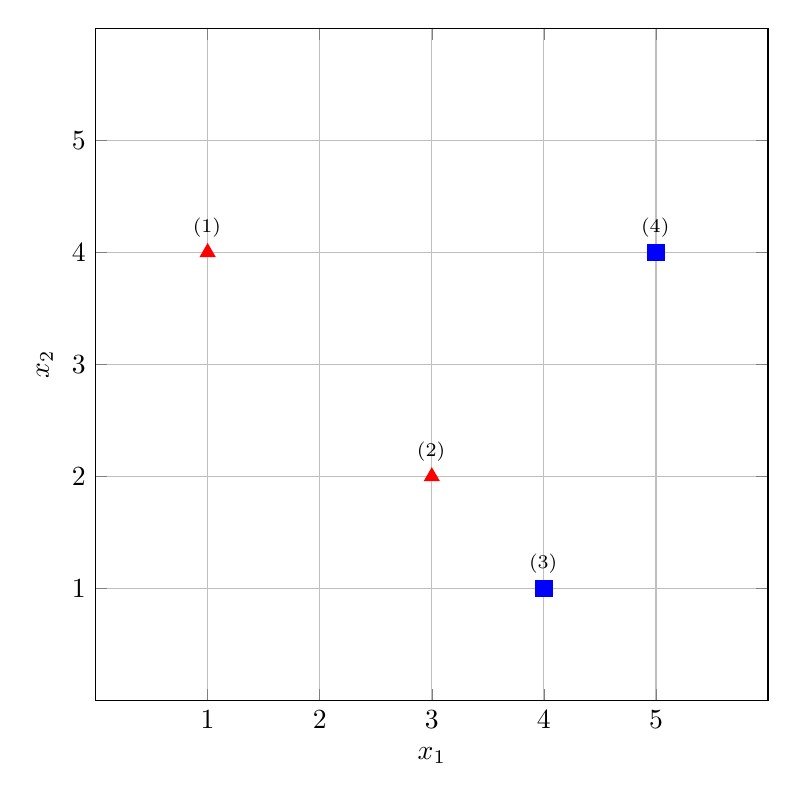
\begin{tikzpicture}
    \begin{axis}[
        scale=1.5, axis equal image, mark options={scale=1.5},
        xmin=0, xmax=6, xtick={1,...,5},
        ymin=0, ymax=6, ytick={1,...,5},
        samples=50, grid=major, xlabel=$x_1$, ylabel=$x_2$]]
        \addplot [
            scatter,
            only marks,
            point meta=explicit symbolic,
            scatter/classes={
                a={mark=square*,blue},
                b={mark=triangle*,red}
            },
            nodes near coords*={$\xv^{(\pgfmathprintnumber[frac]\myvalue)}$},
            visualization depends on={\thisrow{myvalue} \as \myvalue},
        ] table [meta=label] {
            x y label myvalue
            1 4 b 1
            3 2 b 2
            4 1 a 3
            5 4 a 4
        };
    \end{axis}
    \end{tikzpicture} 
\end{center}

\begin{soln}
\begin{center}
    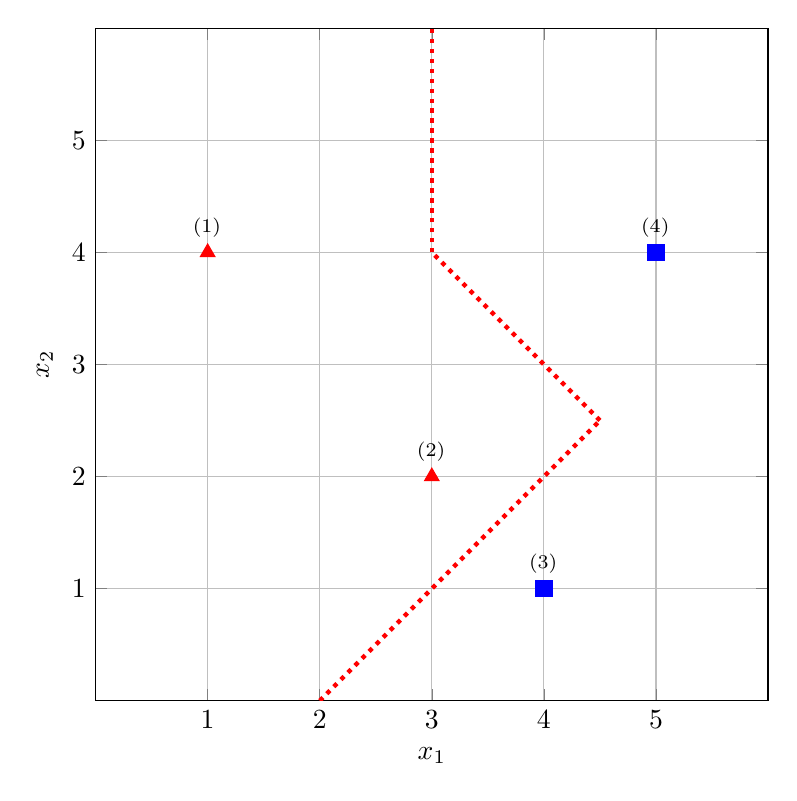
\begin{tikzpicture}
    \begin{axis}[
        scale=1.5, axis equal image, mark options={scale=1.5},
        xmin=0, xmax=6, xtick={1,...,5},
        ymin=0, ymax=6, ytick={1,...,5},
        samples=50, grid=major, xlabel=$x_1$, ylabel=$x_2$]]
        \addplot[red, ultra thick, dotted] coordinates { (2, 0) (4.5, 2.5) };
        \addplot[red, ultra thick, dotted] coordinates { (4.5, 2.5) (3, 4) };
        \addplot[red, ultra thick, dotted] coordinates { (3, 4) (3 ,6) };
        \addplot [
            scatter,
            only marks,
            point meta=explicit symbolic,
            scatter/classes={
                a={mark=square*,blue},
                b={mark=triangle*,red}
            },
            nodes near coords*={$\xv^{(\pgfmathprintnumber[frac]\myvalue)}$},
            visualization depends on={\thisrow{myvalue} \as \myvalue},
        ] table [meta=label] {
            x y label myvalue
            1 4 b 1
            3 2 b 2
            4 1 a 3
            5 4 a 4
        };
    \end{axis}
    \end{tikzpicture}   
\end{center}
\end{soln}
\begin{qauthor}
    Henry
\end{qauthor}

\end{parts}